
                \begin{figure}
                    \centering
                    \begin{tikzpicture}
                        \pgfplotsset{%
                            width=1\textwidth,
                            height=0.4\textheight
                        }
                        \begin{axis}[
                            xlabel={Runs since restart},
                            ylabel={Average dynamic energy (watt)},
                            ymin=0,ymax=70,
                        ]
                        
                            \addplot [mark=none, densely dashed, red]  coordinates {
                            (1, 50.581959309218576)(2, 49.61038875471743)(3, 50.02540589470424)(4, 49.680261087585755)(5, 49.61474108469387)
                            };
                            \addlegendentry{WRK - IPG}
                            
                            \addplot [mark=none, densely dashed, blue]  coordinates {
                            (1, 50.05520471315441)(2, 49.53370095896579)(3, 50.013067368612575)(4, 50.19643007886517)(5, 49.828129143004105)
                            };
                            \addlegendentry{WRK - LHM}
                            
                            \addplot [mark=none, densely dashed, cyan]  coordinates {
                            (1, 40.26202384077937)(2, 40.2932455151716)(3, 36.20059282955928)(4, 41.23661828968479)(5, 40.21968271770776)
                            };
                            \addlegendentry{WRK - CLAMP (win)}
                            
                            \addplot [mark=none, densely dashed, orange]  coordinates {
                            (1, 57.19764983098083)(2, 57.00165164340832)(3, 66.21004004110453)(4, 57.19718608892579)(5, 57.34049914063185)(6, 57.40253642474941)(7, 57.140983667474835)(8, 57.267419084816645)(9, 57.26027791422459)(10, 57.1724159387716)(11, 57.27503186098154)(12, 57.19849623559605)(13, 57.43045034394976)(14, 57.03347688751421)(15, 56.901130170981965)(16, 57.21033764785148)(17, 57.11942779212227)(18, 57.293709254240504)(19, 57.04187945888198)(20, 57.000169254155274)(21, 57.40908459099717)(22, 57.14694833026838)(23, 57.317577493918186)(24, 57.177967278560374)(25, 57.08312806998303)(26, 56.83336498334792)(27, 57.16879940391148)(28, 56.63981918810357)(29, 56.96704807064557)
                            };
                            \addlegendentry{WRK - RAPL}
                            
                            \addplot [mark=none, densely dashed, black]  coordinates {
                            (1, 55.31206096838103)(2, 50.10191246144309)(3, 57.316226683101476)(4, 51.5012766878106)(5, 51.47166924200893)(6, 50.76588789984609)(7, 50.44582359034085)(8, 51.286962607807055)(9, 51.75386417938539)(10, 51.253134769483054)(11, 51.1962751121345)(12, 40.49374473196748)(13, 50.87397347393994)(14, 51.24522018034534)(15, 50.78598420136659)(16, 51.15871585203732)(17, 41.406945986697124)(18, 51.34901650311136)(19, 50.834121040337166)(20, 50.6231501430059)(21, 51.421502231250884)(22, 51.79582574376782)(23, 51.415058928732066)(24, 51.20769337652871)(25, 51.31724419450414)(26, 51.64019970113074)(27, 51.9000210744161)(28, 51.409759727008776)(29, 51.414715940137995)
                            };
                            \addlegendentry{WRK - CLAMP (lin)}
                            
                        \end{axis}
                    \end{tikzpicture} 
                \caption{A graph illustrating the energy consumption of Cores for test case BinaryTrees with regards to how long ago the DUT was restarted, experiment \#2, (with outliers)} \label{fig:BinaryTrees_Cores_iteration_exp2}
                \end{figure}
                